%!TEX root = paper.tex


\section{The HFA Model}

Using our system, a trainer iteratively develops new finite-state automata, whose states encompass behaviors drawn from a behavior library.  An automaton is learned by observing the trainer as he selects various behaviors in various situations.  Once learned, the automaton can then be added as a behavior in the library, and then may be itself used as a state in more complex automata.  In the following, we first describe the hierarchical finite state automaton model, and in the next section we detail our approach for learning the automaton by demonstration from the trainer. 

%Our goal is to learn agent models based on a finite set of atomic behaviors ${\cal B}=\{b_{1},\ldots,b_{n}\}$ and a finite set of features ${\cal F}=\{f_{1},\ldots,f_{n}\}$. Behaviors correspond to pre-implemented actions to which the agent has access in order to build more complex behaviors, while features correspond to the perceptions used for modeling the state of the environment. 


%\subsection{The HFA Model}




\begin{figure}[t]
\begin{center}
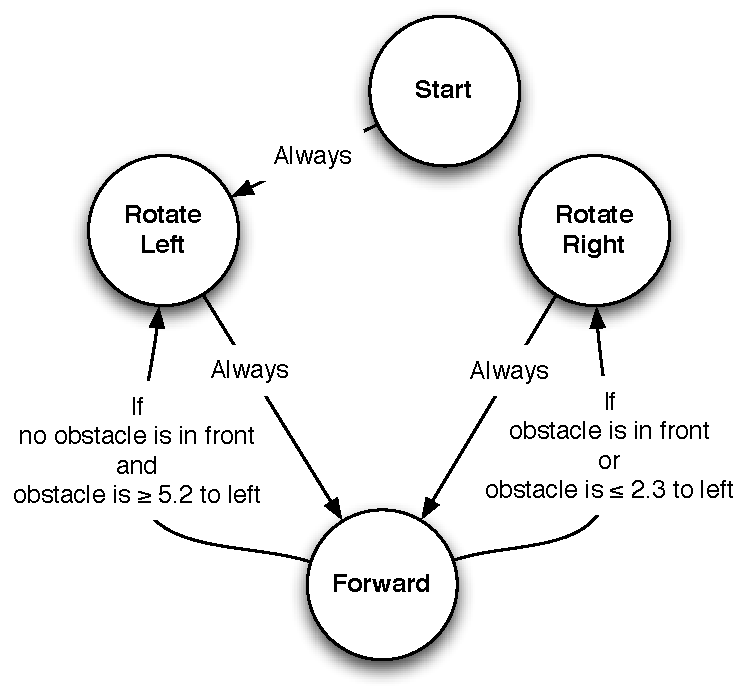
\includegraphics[width=3in]{WallFollower.pdf}
\end{center}
\caption{A simple finite-state automaton for wall following (counter-clockwise).  All conditions not shown are assumed to indicate that the agent remain in its current state.}
\label{fsa}
\end{figure}


\paragraph*{States and Behaviors}
Our HFAs model Moore machines: that is, each state corresponds to a behavior, and when in a state, the HFA performs that behavior.  A behavior may be an atomic behavior or may itself be another HFA, leading to the hierarchical definition of the model.  Atomic behaviors are hard-coded behaviors provided by the system.  For example, the behavior \textsf{rotate-left} might be a basic behavior: when employing this behavior, the agent will spin counterclockwise at some rate.  The HFA always begins in the {\it start state} (\textsf{start}), associated with a special \textsf{idle} behavior, and which always transitions immediately to some other state.  Another special state is the optional {\it done state}, whose behavior simply sets a ``done'' flag and immediately transitions to the start state.  This is used to potentially indicate to higher-level HFAs that the behavior of the current HFA is ``done''.  

 Figure \ref{fsa} shows a simple automaton with four states, corresponding to the behaviors \textsf{start}, \textsf{rotate-left}, \textsf{rotate-right}, and \textsf{forward}.  It may appear at first glance that not all HFAs can be built with this model: for example, what if there were {\it two} states in which the \textsf{rotate-left} behavior needed to be done?  This can be handled by creating a simple HFA which does nothing but transition to the \textsf{rotate-left} state and stay there.  This automaton is then stored as a behavior called \textsf{rotate-left2} and used in our HFA as an additional state, but one which performs the identical behavior to \textsf{rotate-left}. 

\paragraph*{Features}
Transitions from state to state are triggered by observable {\it features} of the environment. One such feature might be \textsf{distance-to-closest-obstacle-on-my-left}.  At any time, this feature yields a non-negative value indicating the distance to such an obstacle.   In our system features presently take three forms: {\it categorical features}, which return unordered values like ``red'' or ``blue'';  {\it continuous features}, which return real-valued numbers (like distances); and {\it toroidal features}, which return real-valued numbers but which are assumed to wrap around in a toroidal fashion (like angles).  Boolean features are typically modeled as categorical features.  One special boolean feature is the \textsf{done} feature, which is true if the current behavior is a lower-level HFA, and if it has triggered its \textsf{done} flag.

\paragraph*{Targets}
Importantly, our approach supports parameterized, general-purpose behaviors and transitions.  Rather than create a behavior called \textsf{go-to-obstacle-number-42}, we can create a behavior called \textsf{go-to(A)}, where \textsf{A} may be specified later.  Similarly, rather than the aforementioned feature \textsf{distance-to-closest-obstacle-on-my-left}, we might instead have the more general feature \textsf{distance-to(B)}.  Thus, this separate notion of features and behaviors from the {\it targets} to which they apply.  For example, a feature or behavior may be either specified with regard to one or more {\it ground targets} (``obstacle 42'' or ``the closest obstacle on my left'')\,---\,resulting in a behavior such as \textsf{go-to}(\textsf{obstacle-42})\,---\,or the target may simply be left unspecified (\textsf{A}), to be bound to a ground target at some later time.  In the latter case, the unbound target is called a {\it parameter}.

When an HFA employs features or behaviors with as-of-yet unbound targets (parameters), it must itself present those parameters when used as a behavior by some higher-level HFA.  Thus HFAs themselves may be parameterized.

%Additionally, when an FSA behavior is created, all parameters of features and behaviors within the FSA must be either bound to ground targets or bound to the FSA's own parameters.  In the latter case the FSA behavior itself becomes a parameterized behavior.

\paragraph*{Transitions}  In traditional finite-state automata, transitions are represented by directed edges between nodes, each labelled with a condition which may or may not be true about the current features of the environment.  Without loss of generality, it's more useful for us to think of a {\it transition function} which maps the current state and the current feature vector into a new state.  The start state always transitions to a specific other state; and the done state always transitions to the start state. 


%Rules are based  on a finite set of features ${\cal F}=\{f_{1},\ldots,f_{n}\}$ that correspond to the perceptions used for modeling the state of the environment.  
%Node transitions take the form of rules which are or are not true about the environment.  We presume that all transitions leaving a node constitute a set of disjoint rules.  If no such rule is true, no transition is triggered and the FSA stays in its present state.  For example, were our FSA presently in the {\it forward} behavior (moving forward), and an obstacle was in front or less than $2.3$ units to the left, we would transition to the {\it rotate right} behavior and start rotating to the right.  On the other hand, if no obstacle was in front and an obstacle was further than $5.2$ units to the left, we would transition to the {\it rotate left} behavior.  Finally, if neither of these were true, we would continue moving forward.  All transitions leaving a given state are collectively embodied in a single {\bf transition} object associated with that state: thus an FSA behavior with \(N\) states also has \(N\) transition objects.  

\paragraph*{Operating the HFA}

Each timestep the HFA is advanced one tick: it performs one step of the behavior associated with its current state, then applies the transition function to determine a new state for next timestep, if any.  When a performed behavior is itself an HFA, this operation is recursive: the child HFA likewise performs one step of {\it its} current behavior, and applies {\it its} transition function.  Additionally, when an HFA transitions to a state whose behavior is an HFA, that HFA is initialized: its initial state is set to the start state, and its ``done'' flag is cleared.

\paragraph*{Formal Model}
 For the purposes of this work, we define the class of hierarchical finite-state automata models  $\cal H$ as the set of tuples \( \langle \mathcal{S}, \mathcal{F}, T, \mathcal{B}, M \rangle\) where:
\begin{itemize}
\item $\mathcal{S} = \{S_0, S_1, \ldots, S_n\}$ is a set of {\it states}, including a distinguished start state $S_{0}$, and possibly also one ``done'' state \(S_*\).  Exactly one state is active at any time.

\item ${\cal F}=\{F_1,F_{2}, \ldots,F_{n}\}$ is a set of  {\it observable features} in the environment. The set of features is partitioned in three disjoint subsets representing categorical (${\cal C}$), continuous (${\cal R}$) and toroidal (${\cal A}$) features. Each $F_{i}$ can assume a value $f_{i}$ drawn from a finite (in the case of ${\cal C}$) or infinite (in the case of ${\cal R}$ and ${\cal A}$) number of possible values.  At any point in time, the present assumed values \(\vec f = \langle f_1, f_2, \ldots, f_n\rangle\) for each of the \(F_1, F_2, \ldots, F_n\) are known as the environment's current {\it feature vector}.

\item \(T: F_1 \times F_2 \times \ldots \times F_n \times \mathcal S \rightarrow \mathcal S\) is a {\it transition function} which maps a given state \(S_i\), and the current feature vector  \(\langle f_1, f_2, \ldots, f_n\rangle\), onto a new state \(S_j\).  The start state and done state have unilateral transitions:  \(\exists S_{k\neq0} \forall \vec f: T(\vec f, S_0) = S_k\), $\forall S_{k} \neq S_{*}\; \forall {\vec f}\; T(\vec f,S_{k})\neq S_{0}$ and \(\forall \vec f: T(\vec f, S_{*}) = S_0\).

%where each edge \(E_i\) is a triple of the form \(\langle S, S', C\rangle\) indicating a current {\it outgoing} state \(S\), a new {\it incoming} state \(S'\), and a {\it condition} \(C\). A {\it condition} \(C\) can be any propositional formula, where propositions  take the form of:
%\begin{itemize}
%\item   $F_{i}=cat$, where $F_{i}\in  {\cal C}$ and $cat$ is a  category of $f$ 
%\item   $F_{i}<v$, where $F_{i}\in  {\cal R}$ and $v \in \mathbb{R}$
%\item   $v_{1}\leq F_{i} <v_{2}$, where $F_{i}\in  {\cal T}$ and $v_1,v_{2} \in \mathbb{R}$
%\end{itemize}

\item ${\cal B}=\{B_1,B_{2},\ldots,B_{n}\}$ is a set of {\it atomic behaviors}.   By default, the special behavior {\sf idle}, which corresponds to inactivity, is in ${\cal B}$, as may also be the optional behavior {\sf done}.

\item \(M: \mathcal{S}\rightarrow {\cal H} \cup {\cal B}\) is a one-to-one mapping function of states to basic behaviors or hierarchical automata.  $M(S_{0})= \textsf{idle}$, and \(M(S_{*})=\textsf{done}$.  \(M\) is constrained by the stipulation that recursion is not permitted, that is, if an HFA \(H\in\cal H\) contains a mapping \(M\) which maps to (among other things) a child HFA \(H'\), then neither \(H'\) nor any of its descendent HFAs may contain mappings which include \(H\).  
\end{itemize}

%A condition can be evaluated over a set of feature values $\langle f_1,\ldots,f_{n}\rangle\in F_{1}\times \ldots \times F_{n}$, i.e. $C(\langle f_1,\ldots,f_{n}\rangle) \in \{\top,\bot\}$.

%\subsubsection*{Learning}
%We presume that for a given state \(S\), all edges with \(S\) as their outgoing state have disjoint and non-conflicting conditions.  Furthermore we may describe all such edges collectively as a {\it transition function} \(T: {\cal S}\times  F_{1}\times \ldots \times F_{n} \rightarrow {\cal S}\) defined as: 
%$$\forall\; S,S'\in{\cal S}\;\;\;\forall\;\langle f_1,\ldots,f_{n}\rangle\in F_{1}\times \ldots \times F_{n}$$ $$T(S,\langle f_1,\ldots,f_{n}\rangle)=S' \iff $$ $$\exists \; \langle S, S', C\rangle\in {\cal E} \mbox{ s.t. } C(\langle f_1,\ldots,f_{n}\rangle) \mbox{ is } true$$

%The learning task consists in learning the transition function $T$.

We further generalize the model by introducing free variables ($G_1,\ldots,G_{n}$) for basic behaviors and features: these free variables are known as {\it targets}.  The model remains unaltered, by replacing behaviors $B_{i}$ with $B_i(G_1,\ldots,G_{n})$ and features $F_{i}$ with $F_{i}(G_{1},\ldots,G_{n})$. The main differences are that the evaluation of the transition function and the execution of behaviors will both be based on ground instances of the free variables.


\section{Learning from Demonstration}

%\subsubsection*{Training}

The above mechanism is sufficient to hand-code HFA behaviors to do a variety of tasks; but our approach was meant instead to enable the learning of such tasks.  Our learning algorithm presumes that the HFA has a fixed set of states, comprising the combined set of atomic behaviors and all previously learned HFAs. Thus, the learning task consists only of learning the transitions among the states: given a state and a feature vector, decide which state (drawn from a finite set) to transition to.  This is an ordinary classification task.  Specifically, for each state \(S_i\) we must learn a classifier \(\vec f \rightarrow \cal S\) whose attributes are the environmental features and whose classes are the various states.  Once the classifiers have been learned, the HFA can then be added to our library of behaviors and itself be used as  a state later on.

Because the potential number of features can be very high, and many unrelated to the task, and because we want to learn based on a very small number of samples, we wish to reduce the dimensionality of the input space to the machine learning algorithm.  This is done by allowing the user to specify beforehand which features will matter to train a given behavior.  For example, to learn a Figure-8 pattern around two unspecified targets A and B, the user might indicate a desire to use only four parameterized features: \textsf{distance-to(A)}, \textsf{distance-to(B)}, \textsf{direction-to(A)}, and \textsf{direction-to(B)}.  During training the user temporarily binds A and B to some ground targets in the environment, but after training they are unbound again.  The resulting learned behavior will itself have two parameters (\textsf{A} and \textsf{B}), which must ultimately be bound to use it in any meaningful way later on.   

The training process works as follows.  The HFA starts in the ``start'' state (idling).  The user then directs the agent to perform various behaviors in the environment as time progresses.   When the agent is presently performing a behavior associated with a state \(S_i\) and the user chooses a new behavior associated with the state \(S_j\), the agent transitions to this new behavior and records an {\it example}, of the form \(\langle S_i, \vec{f}, S_j\rangle\), where \(\vec{f}\) is the current feature vector.  Immediately after the agent has transitioned to \(S_j\), it turns out to be often helpful to record an additional example of the form \(\langle S_j, \vec{f}, S_j\rangle\).  This adds at least one ``default'' (that is, ``keep doing state \(S_j\)'') example, and is nearly always correct since in that current world situation the user, who had just transitioned to \(S_j\) would nearly always want to stay in \(S_j\) rather than instantaneously transition away again.

At the completion of the training session, the system then builds transition functions from the recorded examples.  For each state \(S_k\), we build a decision tree \(D_{S_k}\) based on all examples where \(S_k\) is the first element, that is, of the form \(\langle S_k, \vec{f}, S_i\rangle\).  Here, \(\vec{f}\) and \(S_i\) form a data sample for the classifier: \(\vec{f}\) is the input feature and \(S_i\) is the desired output class.  If there are no examples at all (because the user never transitioned from \(S_k\)), the transition function is simply defined as always transitioning to back to \(S_k\).

At the end of this process, our approach has built some \(N\) decision trees, one per state, which collectively form the transition function for the HFA.  After training, some states will be unreachable because the user never visited them, and so no learned classification function ever mapped to them.  These states may be discarded.  The agent can then be left to wander about in the world on its own, using the resulting HFA.

%We note that equating behaviors with states is not sufficient for a general Moore-machine FSA: in a real Moore machine, multiple states may perform the same behavior.  Thus if there is only one ``go to A'' button, two states which require going to A will require special handling.  Our approach deals with this in one of two ways.  First, our approach might permit multiple buttons which do the same behavior (but which represent separate states in the FSA).  Second, it's straightforward to train a simple one-state FSA which simply does ``go to A''.  This FSA can then be named, say, ``go to A number 2'' and be included along with ``go to A'' for the user to use: they're different states (technically different behaviors) but ultimately do exactly the same thing.
%
%\paragraph{Toroidal Features -pie slice} We pause to note how we implemented toroidal features in decision trees.  Because angular regions are so common (and are toroidal), toroidal features are important.  The decision tree performs splits on toroidal regions much like it performs splits on continuous regions: by sorting the data by feature value and then finding the lowest-information split.  However whereas continuous splits involve finding a single split point \(A\) and breaking the examples into values \(< A\) versus \(\geq A\), toroidal splits instead involve finding {\it two} split points \(A\) and \(B\), with \(A < B\), and breaking the data into values \(v\) for which \(A \leq v < B\) and values which are either \(< A\) or \(\geq B\).  We term these groups ones which are ``inside'' and ``outside'' the split respectively.  We realize the cost of finding not one but two split values increases the computational complexity of finding an optimal split point by an additional \(O(n)\).  Though we doubt our approach here is original (and have not looked very hard), we have so far not found any other use of toroidal splits in the decision tree literature.

Though in theory many classification algorithms are applicable (such as K-Nearest-Neighbor or Support Vector Machines), in our experiments we chose to use a variant of the C4.5 Decision Tree algorithm~\cite{c4.5} for several reasons:
\begin{enumerate}
\item Many areas of interest in the feature space of our agent approximately take the form of rectangular regions (angles, distances, etc.).
\item Decision trees nicely handle various kinds of data: in our case, we used categorical, real-valued, and toroidal data (the latter requiring so-called ``pie-slice'' decision tree splits). 
\item Decision trees are particularly adept at handling unscaled dimensions in the feature space.  In our case, we would otherwise be faced with asking how many units of distance was equivalent to a degree of angle, or a change from ``true'' to ``false''.
\end{enumerate}

During the implementation and the evaluation of the decision tree learning algorithm, we found out that in some cases we would not want a deterministic classification. For example, when performing a wall-following behavior, we'd need to turn left some {\it percentage} of time. For this reason, we employed leaf nodes in the decision tree which yielded a probability distribution over classes rather than the single class typically generated through majority-value.